\documentclass[tikz]{standalone}
\begin{document}
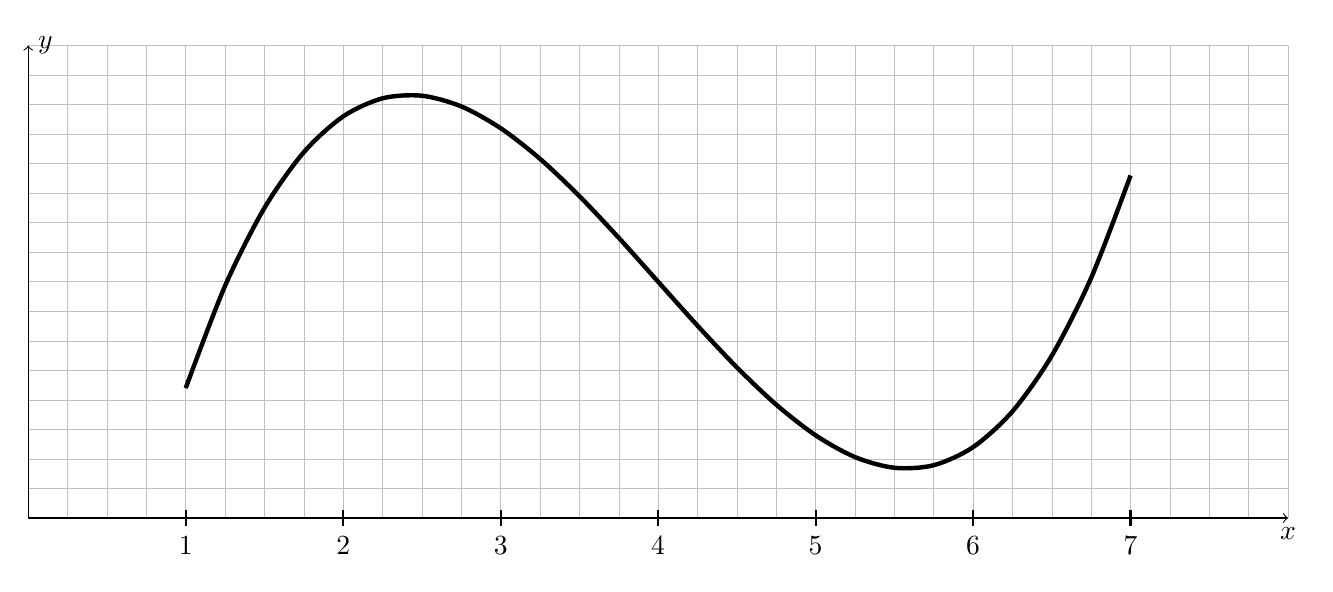
\begin{tikzpicture}[xscale = 2,yscale=1.5]
\draw[white,fill=white] (0,0) rectangle (3,4);
 \draw[very thin,color=darkgray,step=1.0] (0,0) grid (8,4);
 \draw[very thin,color=lightgray,step=0.25] (0,0) grid (8,4);

\draw[->] (0,0) -- (8,0) node[below] {$x$};
\draw[->] (0,0) -- (0,4) node[right] {$y$};
     
% draw curve
\draw [ultra thick,smooth,variable=\x] plot [domain=1:7] (\x,{0.2*(pow(\x-4,3)) - 1.5*(\x-4) + 2});

% tick marks
\foreach \x in {1,...,7} 
	\draw [thick] (\x cm,2pt) -- (\x cm,-2pt) node[below] {$\x$};

\end{tikzpicture}
\end{document}
